\chapter{I-Mode Pedestal Stability Modeling}\label{ch:ImodeModeling}

Large, uncontrolled Edge-Localized Modes (ELMs -- see \cref{sec:hcr_elmy}) in ITER-scale operation are expected to drive unacceptable levels of pulsed heat loading and erosion damage to plasma-facing materials \cite{Loarte2003,Federici2003}.  As such, avoiding or mitigating large ELMs is a major focus of research in high-performance regimes: approaches include active ELM control in H-mode (\cref{subsec:hcr_elmy_control}) and inherently ELM-suppressed regimes (\cref{sec:hcr_elmsuppressed}).  To these we add the I-mode (\cref{sec:hcr_imode}), which appears to be naturally stable against large, deleterious ELMs in addition to its other beneficial properties (see \cref{ch:ImodePedestal}).

Confidence in plans for high-performance operation on ITER- and reactor-scale devices requires a predictive model for the pedestal structure and stability, to optimize fusion performance and ELM control or avoidance.  Recent cooperative efforts among theory, modeling, and experiment \cite{Groebner2013} have resulted in such a model for ELMy H-modes, termed EPED \cite{Snyder2009,Snyder2011}, detailed in \cref{sec:mod_eped}.  The EPED model combines constraints from peeling-ballooning MHD stability (\cref{sec:mod_pb}) \cite{Wilson2002,Snyder2004,Wilson2006}\gnote{cites?} and kinetic-ballooning turbulence (\cref{sec:mod_turbulence}) \cite{Snyder1999,Candy2005,Snyder2001}.  The EPED model has been successfully implemented in ELMy H-mode on a number of machines, including DIII-D \cite{Snyder2009,Snyder2011}, JT-60U \cite{Snyder2009}, C-Mod \cite{Walk2012}, and KSTAR \cite{Han2013}, as well as in QH-mode \cite{Snyder2012}; small/no-ELM regimes (EDA H-mode, type-II and type-III ELMy H-modes) have been shown to be stable against the drive identified in the EPED model \cite{Snyder2009}.

In this chapter, we apply the EPED approach to I-mode, examining the stability of the I-mode pedestal against peeling-ballooning MHD and kinetic-ballooning turbulence \cite{Walk2014}.  This is compared to the observed lack of large ELMs in I-mode, with a goal of examining the parameter space in which ELM-free stationary operation with I-mode is possible.  We also examine the stability and edge behavior of cases in which small, intermittent ELM-like events are observed in I-mode.\nicesectionending

\section{MHD Stability -- ELITE}\label{sec:imode_elite}

\begin{figure}[p]
 \pushtooutside
 \ffigbox[\FBwidth]{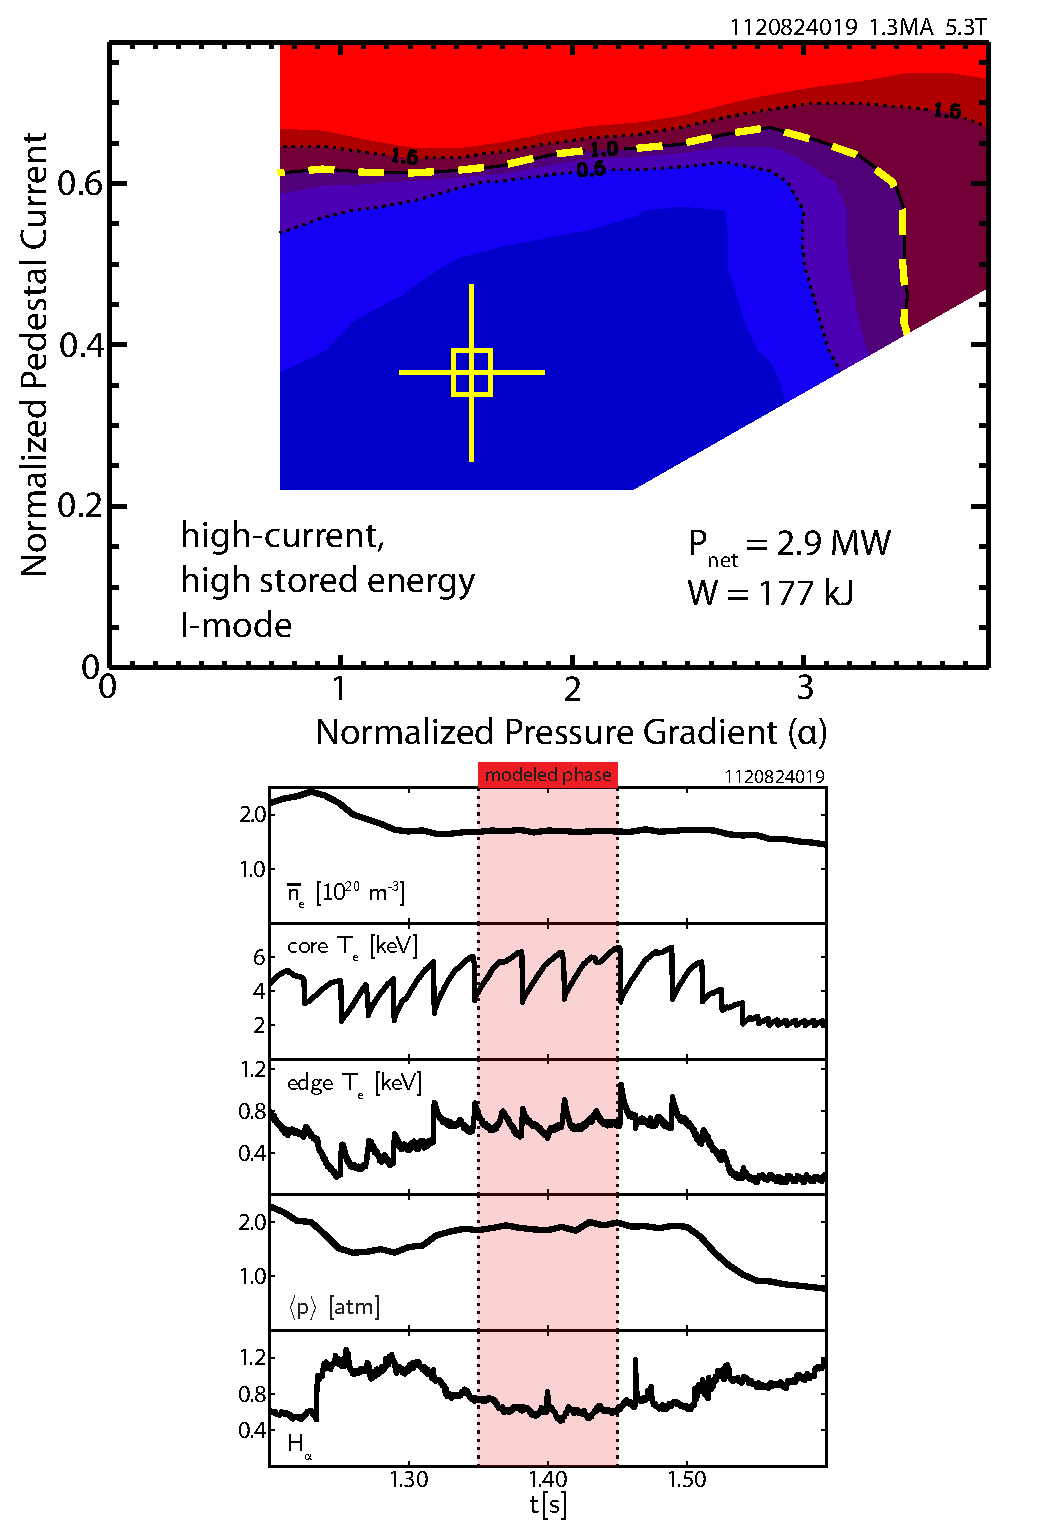
\includegraphics[width=150mm]{graphics/IModeModeling/1120824019_ELITE_stitch_vert.pdf}}{\caption[I-mode pedestal MHD stability contour generated by ELITE.]{MHD stability contour for a high-current ($\SI{1.3}{\mega\ampere}$), high-performance I-mode generated by the ELITE code.  The experimental measurement is shown by the crosshair, with the stability boundary indicated by the yellow dashed line.  Parameters for the modeled phase of the discharge are shown below.  The I-mode pedestal is observed to be far from both the peeling and ballooning MHD stability boundaries.}\label{fig:imode_elite_noelm}}
\end{figure}

The triggering of large ELMs in H-mode has been identified with the interaction between pressure-driven ballooning and current-driven edge kink/peeling MHD instabilities (the latter is typically referred to as a ``peeling'' mode to distinguish it from similarly current-driven core kink modes) in the pedestal \cite{Wilson2002,Snyder2004,Wilson2006}.  Numerical studies of these instabilities using the ELITE code \cite{Wilson2002,Snyder2003}, detailed in \cref{subsec:mod_elite}, have proven quite successful in capturing the physics of the ELM trigger.

At its simplest, ELITE

An ELITE calculation for the I-mode pedestal is shown in \cref{fig:imode_elite_noelm}, along with parameters (line-averaged density, core and edge $T_e$, global-average pressure, and $H_\alpha$ emission) for the modeled phase of the discharge.

\begin{figure}[p]
 \pushtooutside
 \ffigbox[\FBwidth]{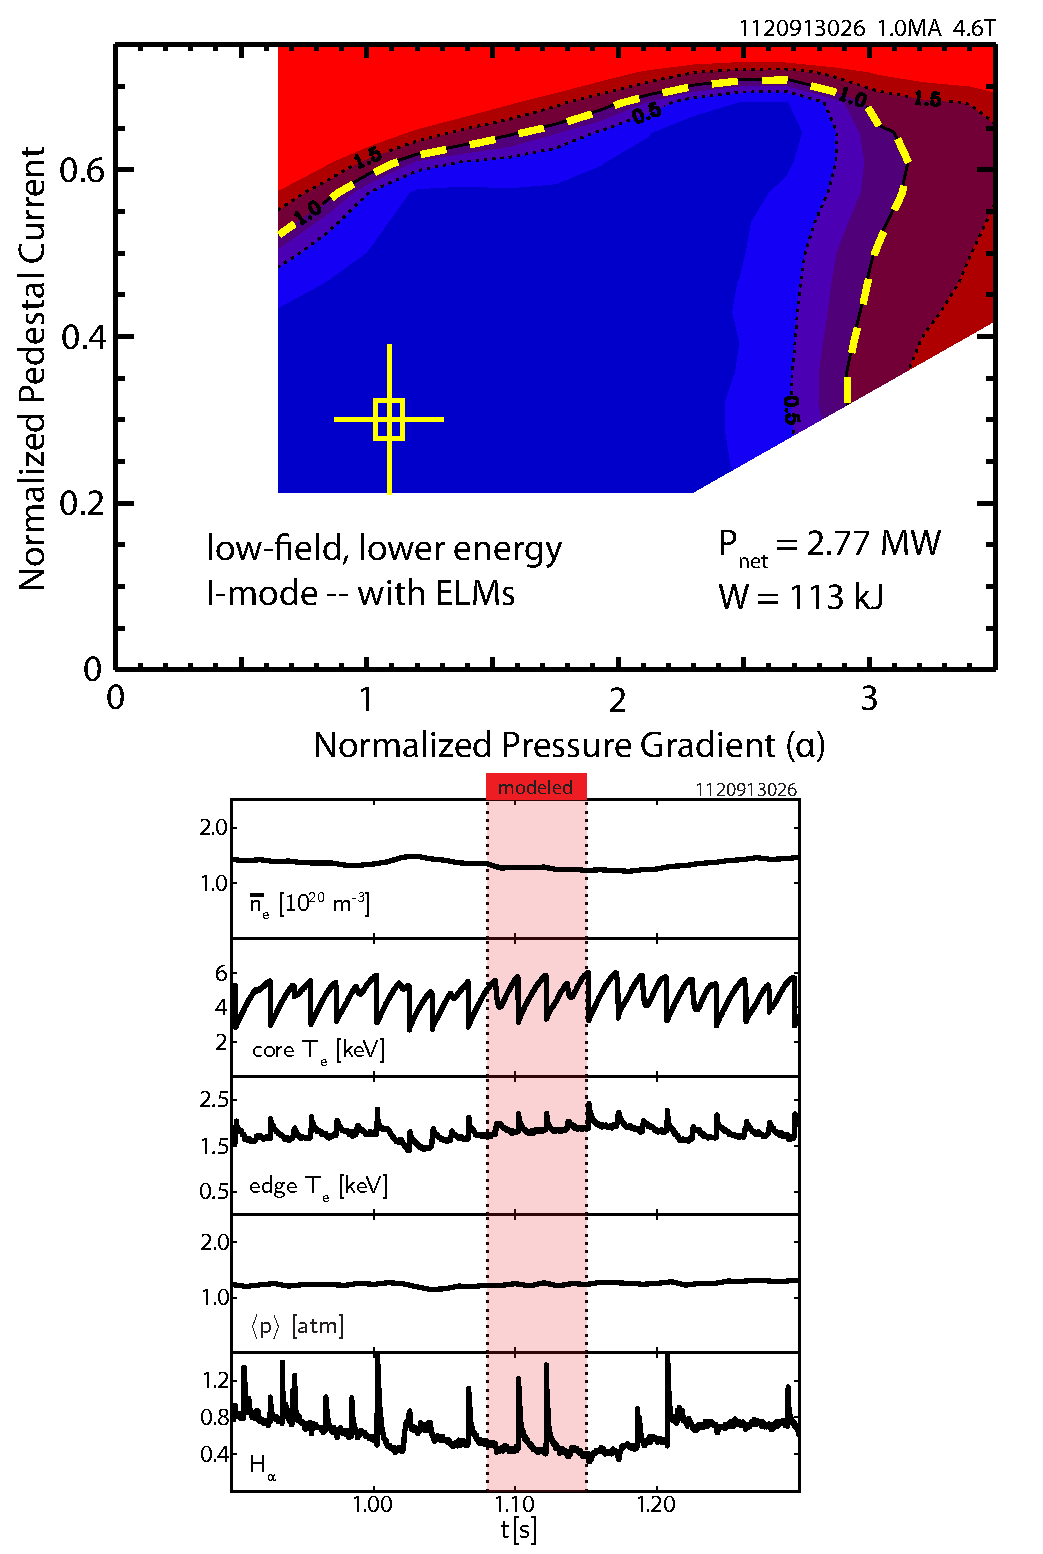
\includegraphics[width=150mm]{graphics/IModeModeling/1120913026_ELITE_stitch_vert.pdf}}{\caption[]{}\label{fig:imode_elite_stelm}}
\end{figure}

\begin{figure}
 \pushtooutside
 \ffigbox[\FBwidth]{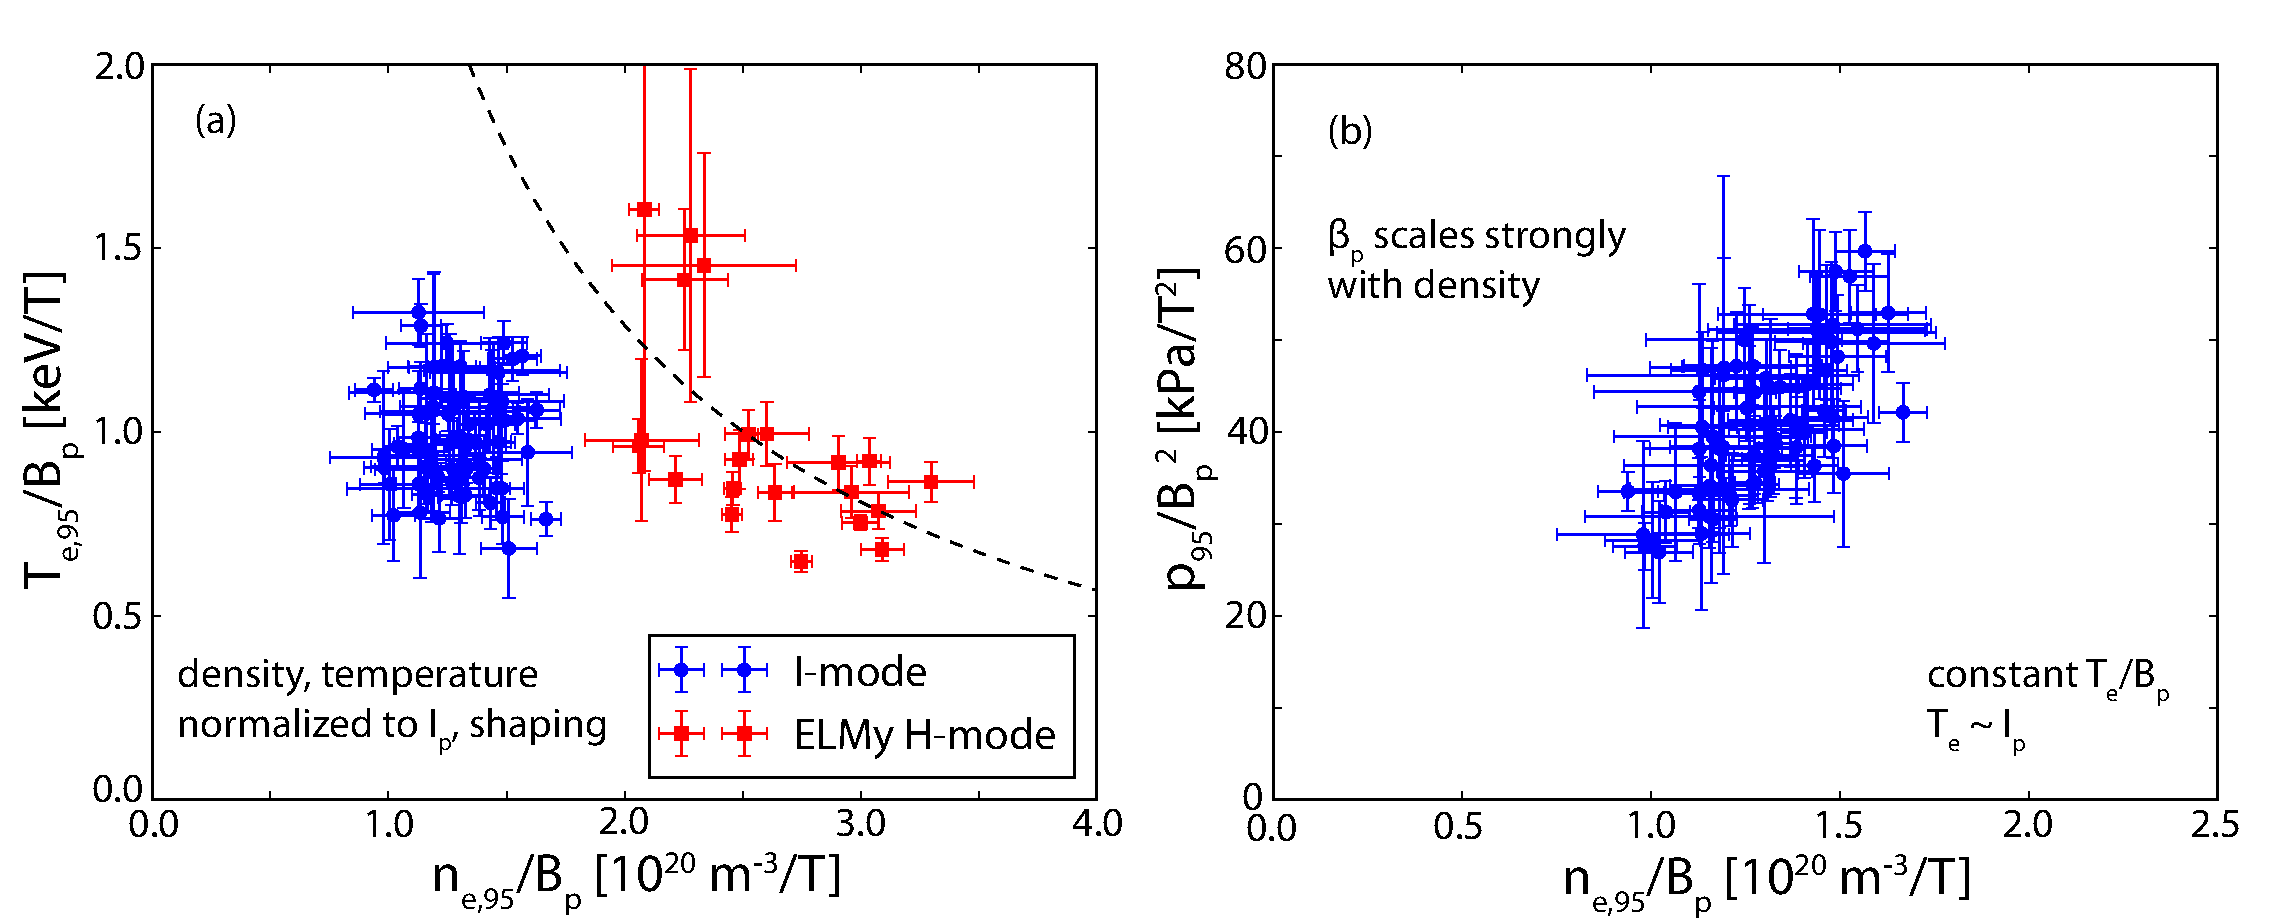
\includegraphics[width=150mm]{graphics/IModeModeling/neBp_stitch.pdf}}{\caption[]{}\label{fig:neBp_stitch}}
\end{figure}

\nicesectionending

\section{KBM and Infinite-$n$ MHD Stability}\label{sec:imode_baloo}

\begin{figure}
 \pushtooutside
 \ffigbox[\FBwidth]{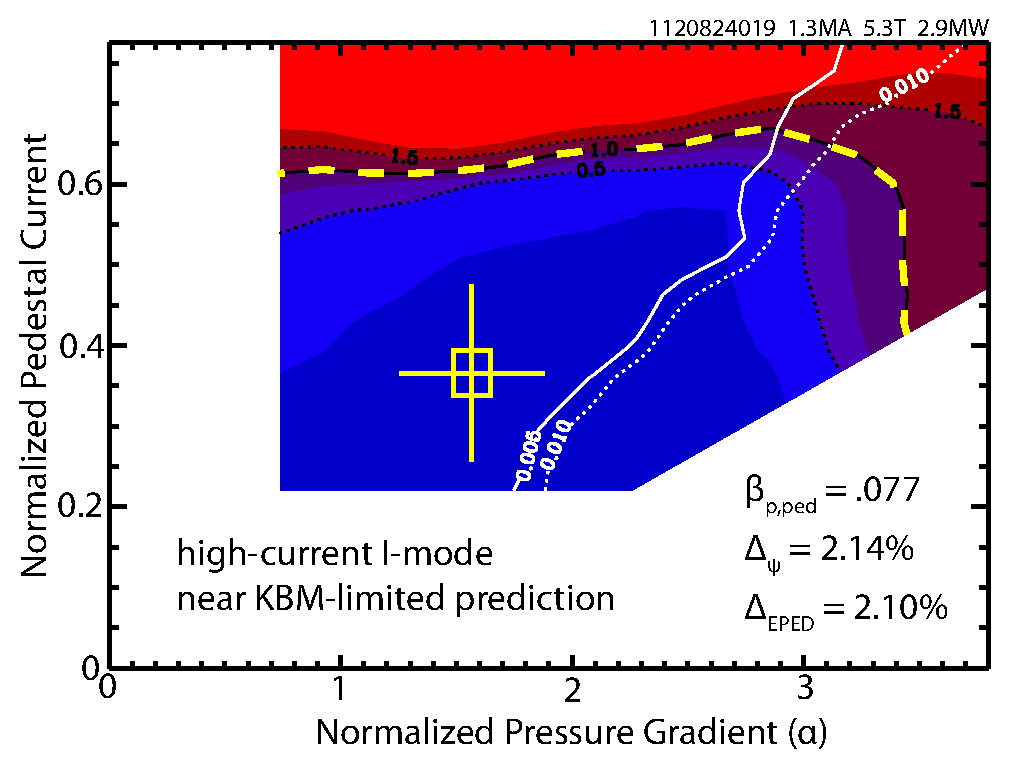
\includegraphics[width=150mm]{graphics/IModeModeling/1120824019_1400n5_35_gamws16_bal.pdf}}{\caption[]{}\label{fig:imode_baloo_noelm}}
\end{figure}

\begin{figure}
 \pushtooutside
 \ffigbox[\FBwidth]{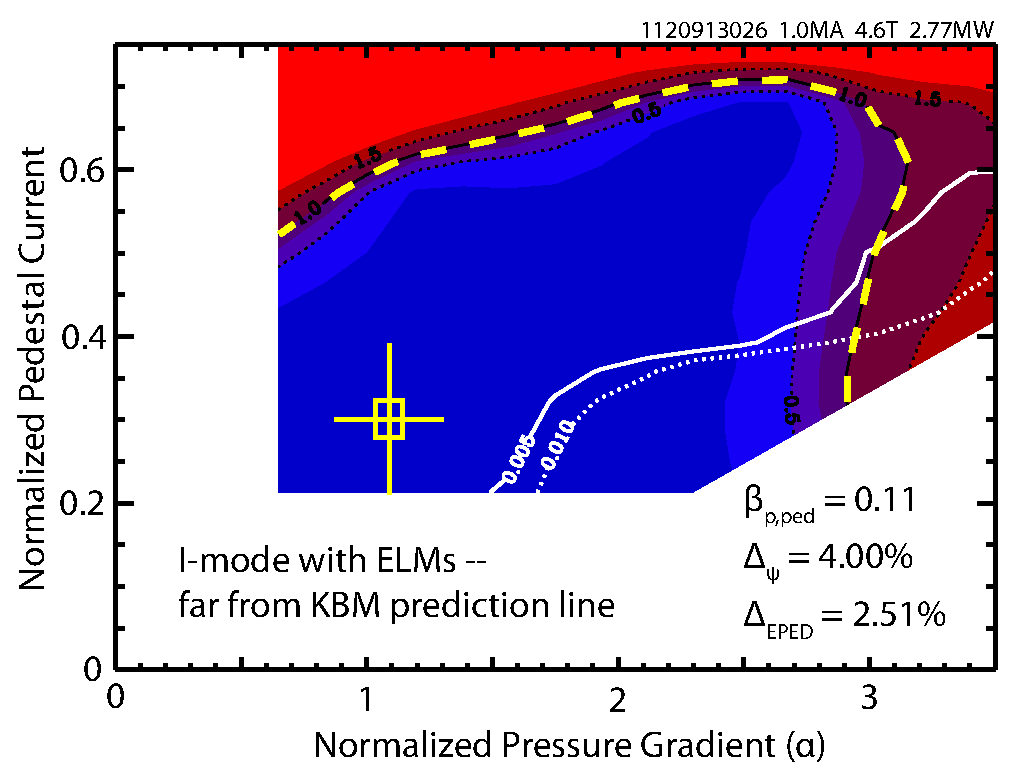
\includegraphics[width=150mm]{graphics/IModeModeling/1120913026_1186n5_35_bal_jalpha.pdf}}{\caption[]{}\label{fig:imode_baloo_stelm}}
\end{figure}

\nicesectionending

\section{Intermittent ELMs in I-Mode}\label{sec:imode_elms}

\begin{figure}
 \pushtooutside
 \ffigbox[\FBwidth]{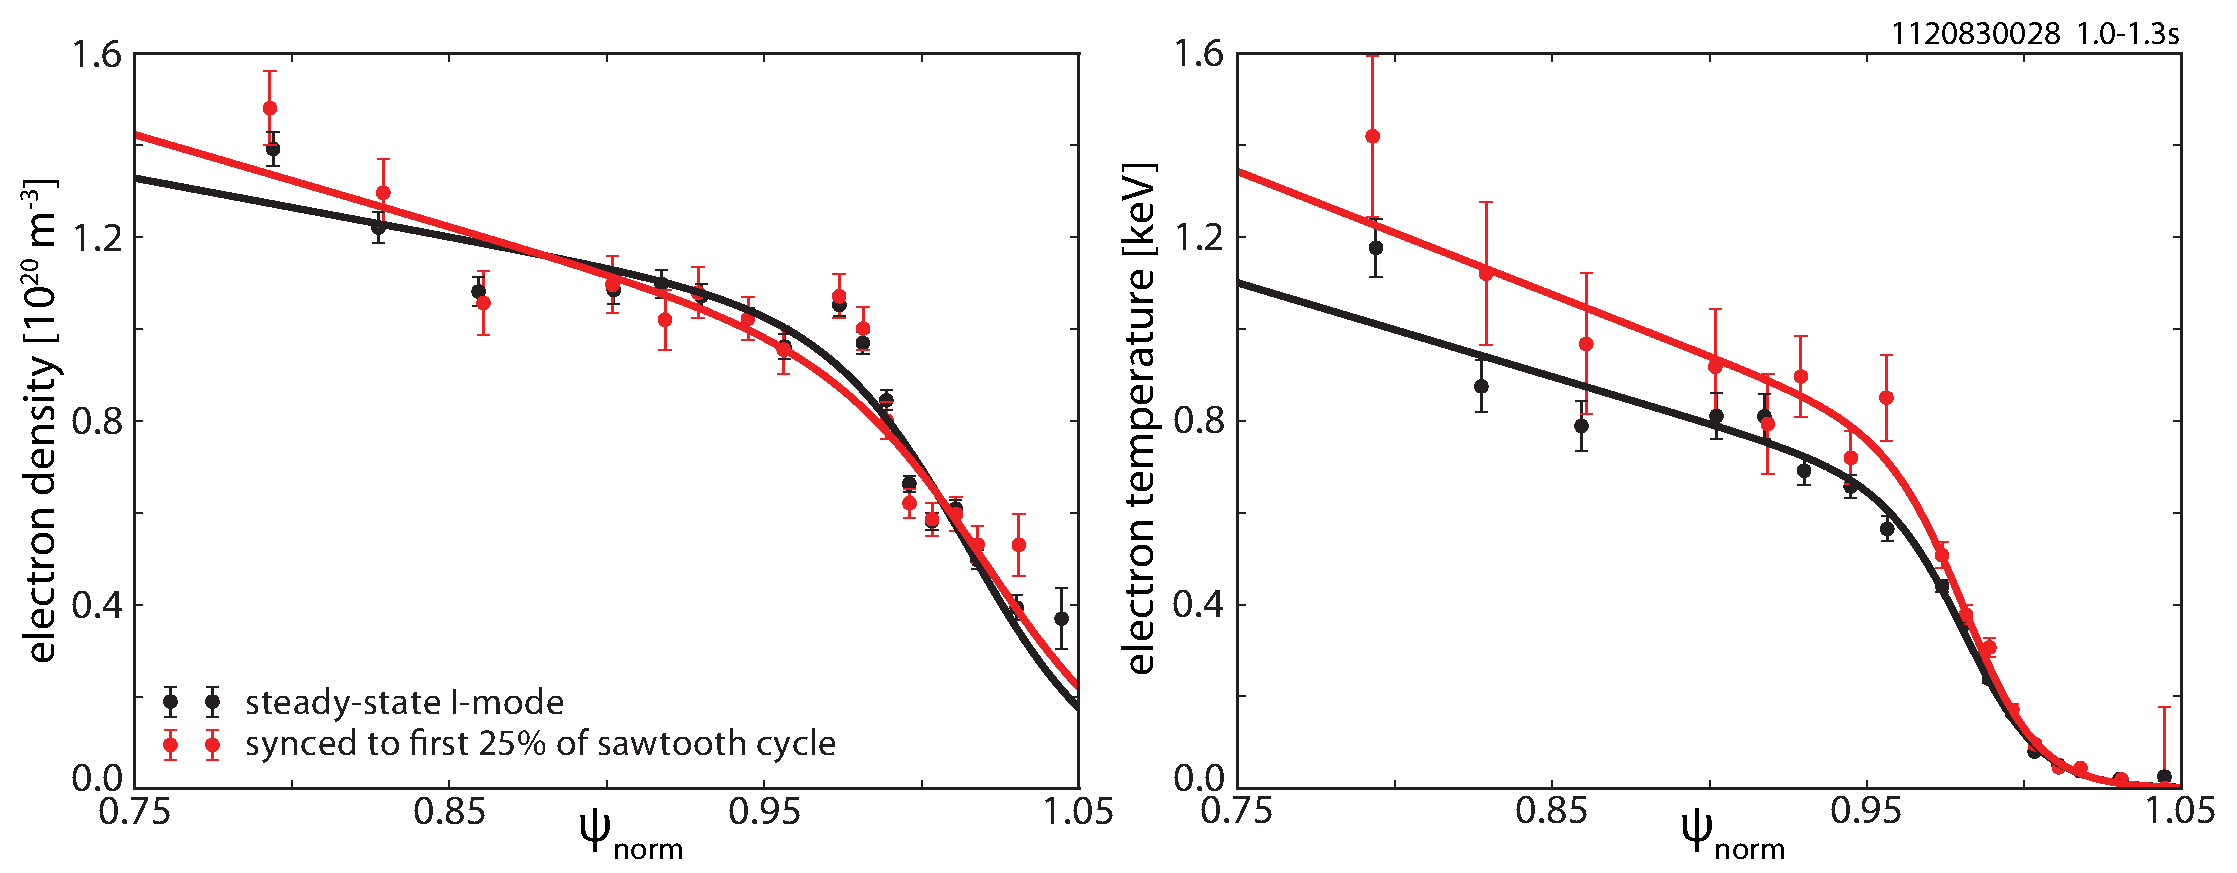
\includegraphics[width=150mm]{graphics/IModeModeling/1120830028_prof_stbin.pdf}}{\caption[]{}\label{fig:prof_stbin}}
\end{figure}

\begin{figure}
 \pushtooutside
 \ffigbox[\FBwidth]{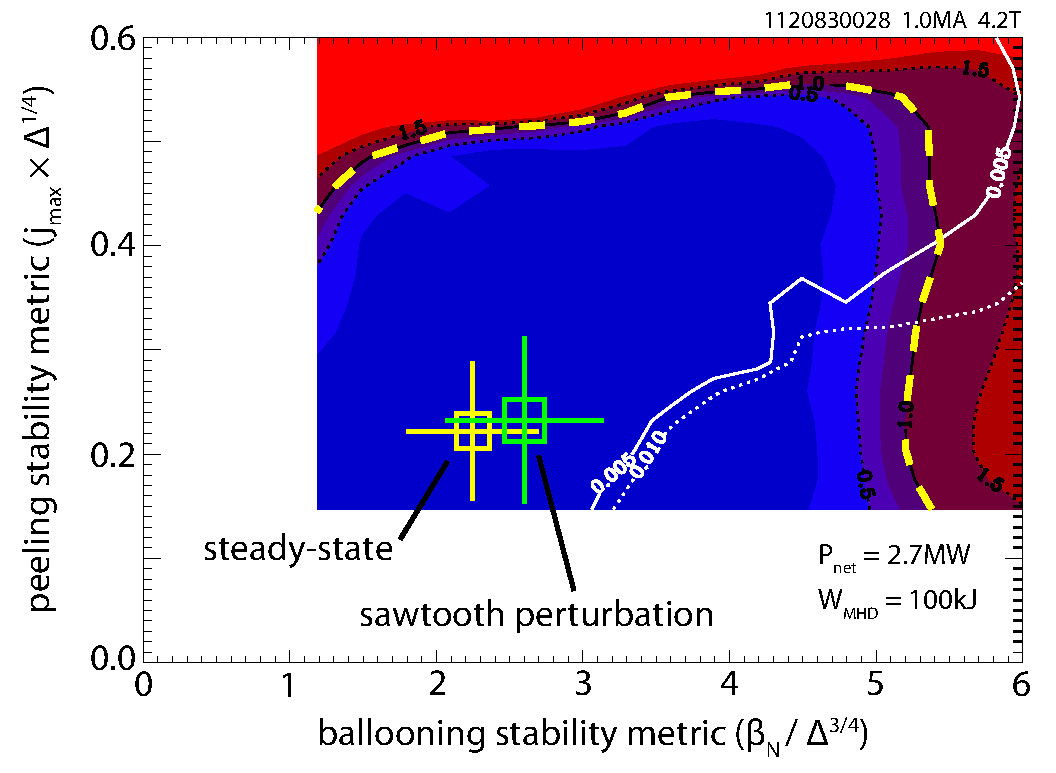
\includegraphics[width=150mm]{graphics/IModeModeling/1120830028_stbin_elite.pdf}}{\caption[]{}\label{fig:imode_stbin}}
\end{figure}

\begin{figure}
 \pushtooutside
 \ffigbox[\FBwidth]{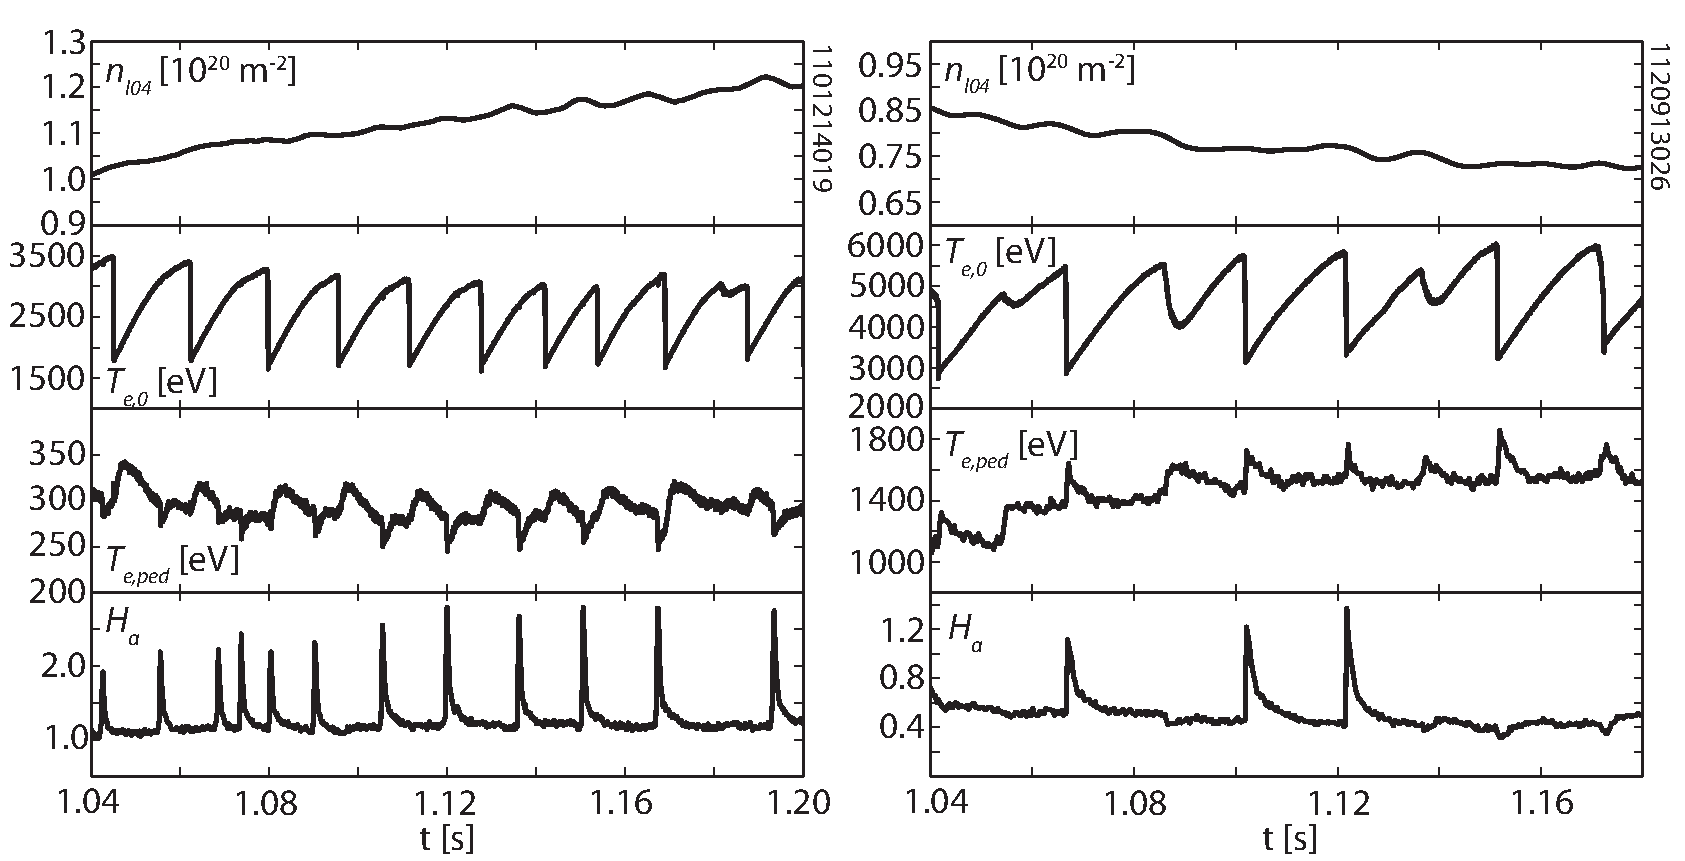
\includegraphics[width=150mm]{graphics/IModeModeling/trace_elmy_imode.pdf}}{\caption[]{}\label{fig:trace_elmy_imode}}
\end{figure}

\begin{figure}
 \pushtooutside
 \fcapside[60mm]{\caption[]{}\label{fig:trace_imode_welms}}{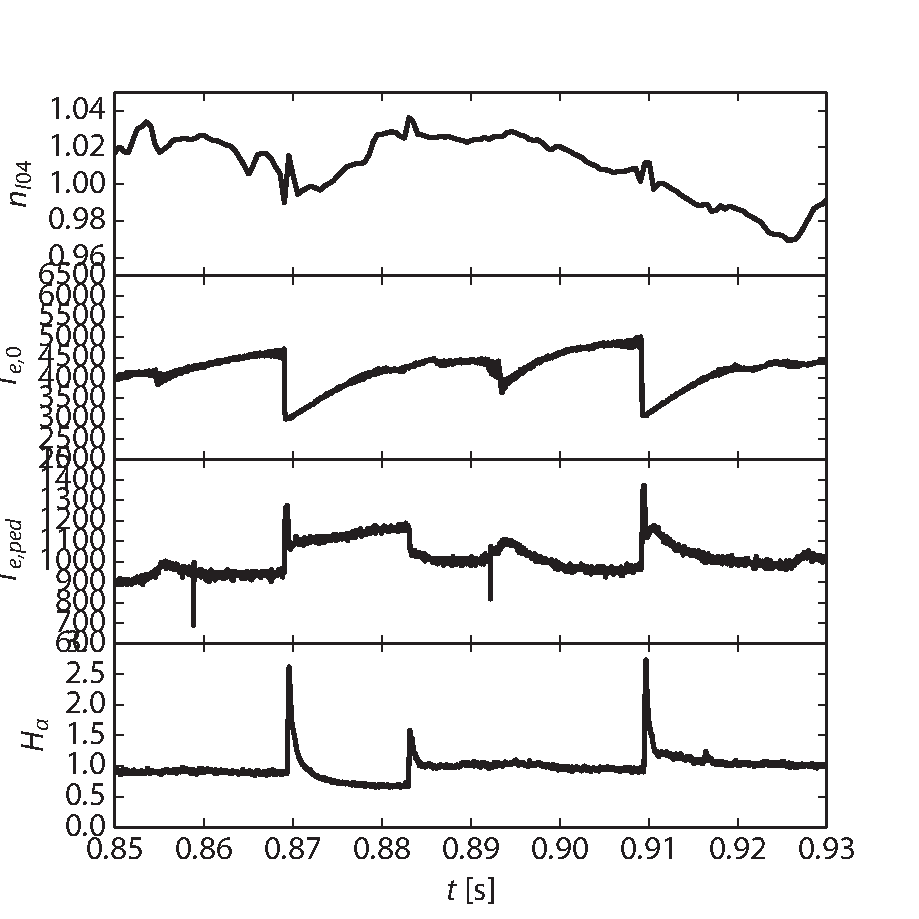
\includegraphics[width=100mm]{graphics/IModeModeling/trace_imode_welms_2.pdf}}
\end{figure}

\begin{figure}[p]
 \pushtooutside
 \ffigbox[\FBwidth]{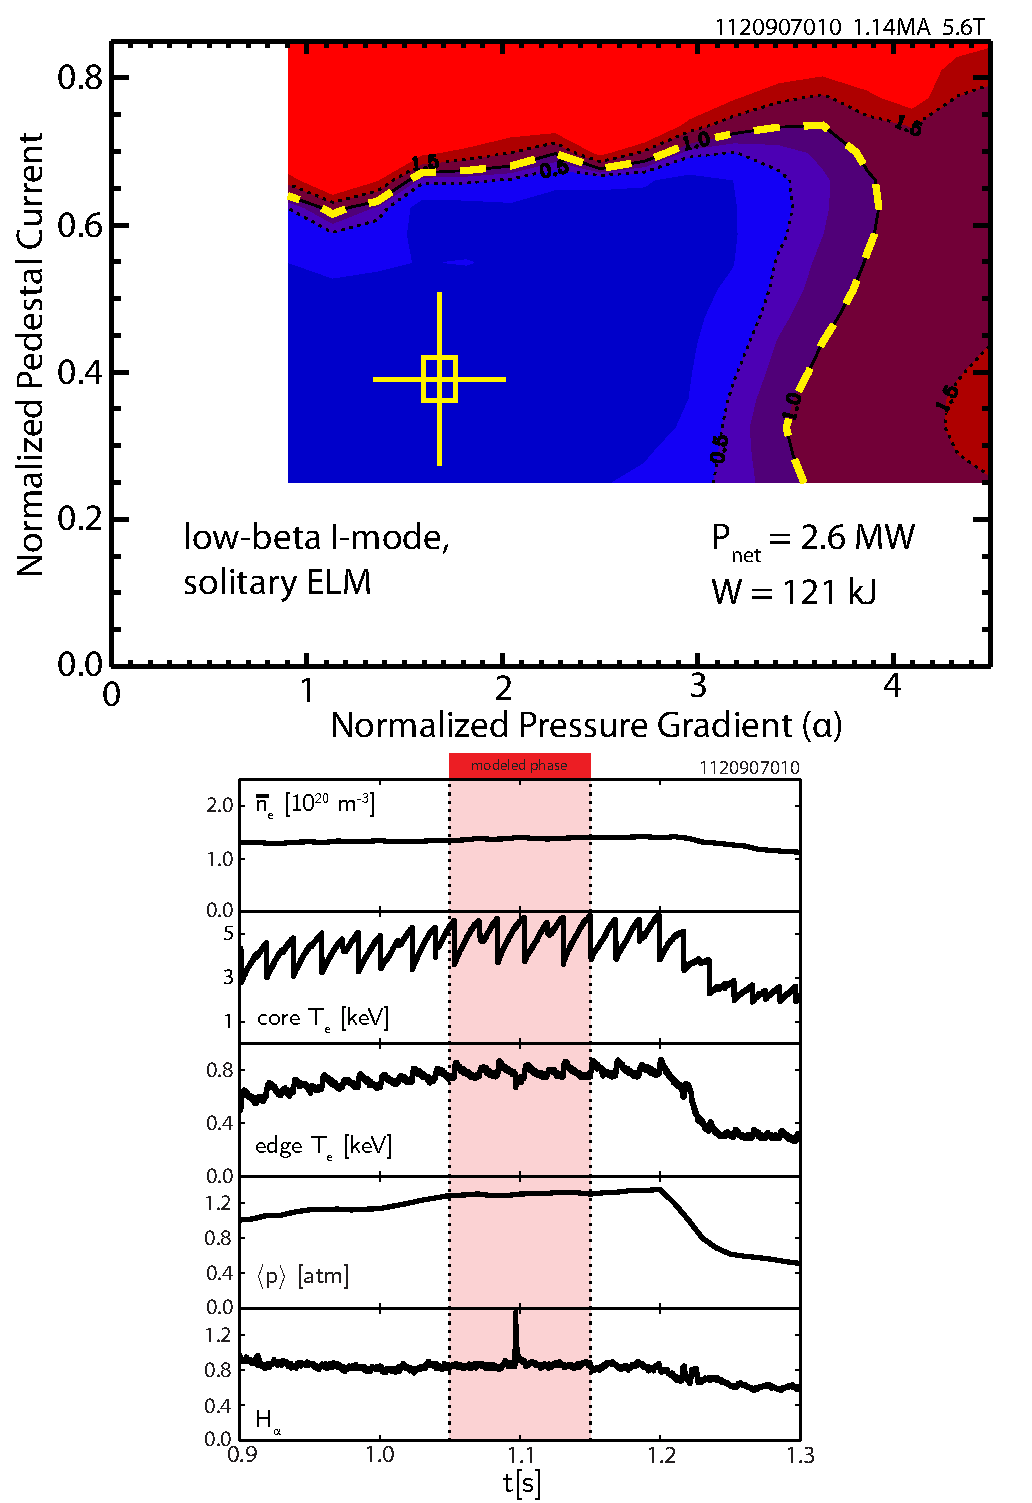
\includegraphics[width=150mm]{graphics/IModeModeling/1120907010_ELITE_stitch_vert.pdf}}{\caption[]{}\label{fig:imode_elite_nonstelms}}
\end{figure}

\begin{figure}
 \pushtooutside
 \ffigbox[\FBwidth]{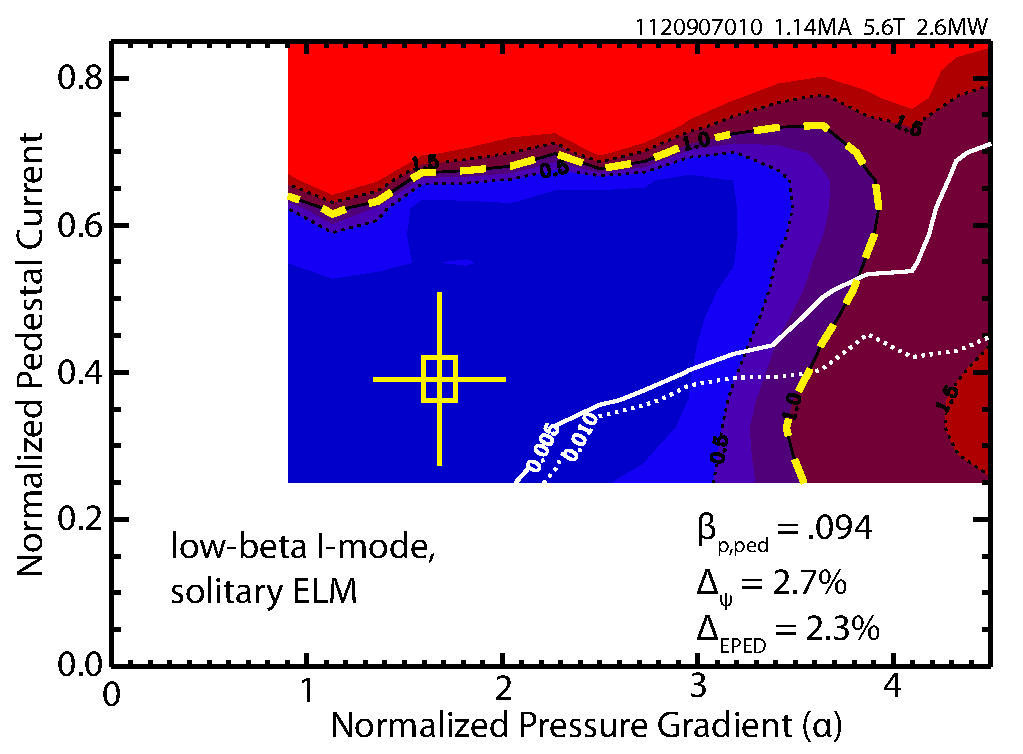
\includegraphics[width=150mm]{graphics/IModeModeling/1120907010_1100n5_35_gamws16_bal.pdf}}{\caption[]{}\label{fig:imode_baloo_nonstelms}}
\end{figure}

\nicechapterending

\bibliographystyle{../plainurl}
\bibliography{../references}